\chapter{Overview of Methodology} 
\label{chapter-outline}

\section{Main objective}

The main objective of our project is to study the manifold structure of biological and artificial neural networks. This objective is equivalent to generating the underlying neural manifolds from data that are obtained from biological and artificial neural networks respectively. In what follows, we will give an overview of the methodology according to the following quesions:
\begin{itemize}
    \item What is a neural manifold?
    \item How to generate the neural manifold?
    \item What can we analyze from the neural manifold?
\end{itemize}


\section{What is a neural manifold?}
Before explaining the idea behind ``neural manifold" in the context of neuroscience, we first introduce the general concept of a manifold as a mathematical object.

\begin{defn}[Homeomorphism]
A continuous map $f: X \to Y$ be a function between topological spaces $X$ and $Y$. If $f$ is bijective, then the inverse $f^{-1}$ exists. If both $f$ and $f^{-1}$ are continuous, then $f$ is a \underline{homeomorphism}. The two topological spaces, $X$ and $Y$, are said to be \underline{homeomorphic} if there exists a homeomorphism between $X$ and $Y$. 
\end{defn}
    \begin{defn}[Manifold]
   In brief, a \underline{real $n$-dimensional manifold} is a topological space $\mathcal{M}$ for which every point $x\in\mathcal{M}$ has a neighborhood homeomorphic to Euclidean space $\RR^n$.
    \end{defn}
   \begin{figure}[H]
      \centering
     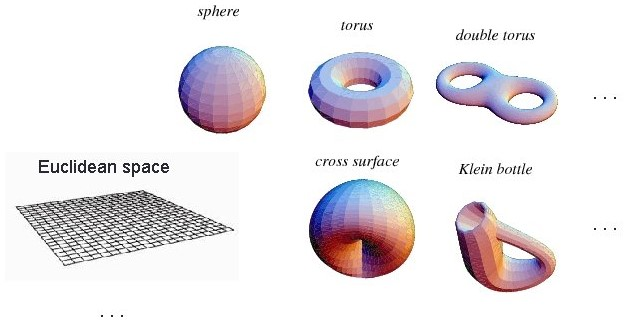
\includegraphics[width=0.4\textwidth]{presentation/manifold.jpg}
     \caption{Examples of $2$-dimensional manifolds.}
    \end{figure} 
            
Our approach to study the neural population response via the neural manifold is based on the premise of ``the Manifold Hypothesis," which states that real-world high-dimensional data lie on a low-dimensional manifold embedded within the high-dimensional space. (\cite{deepai_2019}) The original representation of data has a large degree of freedom, that is, the number of variables that are really necessary to describe the data is much smaller than the number of variables in the original representation. 

% We can illustrate this hypothesis with image data: an image is high-dimensional since the number of dimensions of an image equals the number of pixels. Each image can be reparameterized with much smaller number of variables after applying appropriate feature extraction algorithms. 

% main idea behind manifold learning:
In the context of neuroscience, neural spiking data are usually high-dimensional due to the kind of data representation (the peristimulus, or PSTH, diagrams) determined by the lab instrument. However, it has been shown that the neural connections constrain the possible patterns of neural population activity (\cite{okun_diverse_2015}, \cite{sadtler_neural_2014}, \cite{tsodyks_attractor_1999}) and that the possible patterns are confined to a low-dimensional manifold (\cite{stopfer_intensity_2003},  \cite{yu_gaussian-process_2009}) spanned by a few independent patterns that are called ``neural modes." (\cite{gallego_neural_2017})

We call this underlying low-dimensional manifold the ``\textbf{neural manifold}." The distance between a pair of points on the neural manifold indicate how similar their firing patterns are in response to a given visual stimulus. Intuitively we can understand the neural manifold as a collection of clusters of neurons grouped by their firing patterns in response to a given visual stimulus. Figure \ref{fig:neural-manifold-eg} shows an example of a neural manifold generated from neural spiking data. 

 
      \begin{figure}[H]
        \centering
      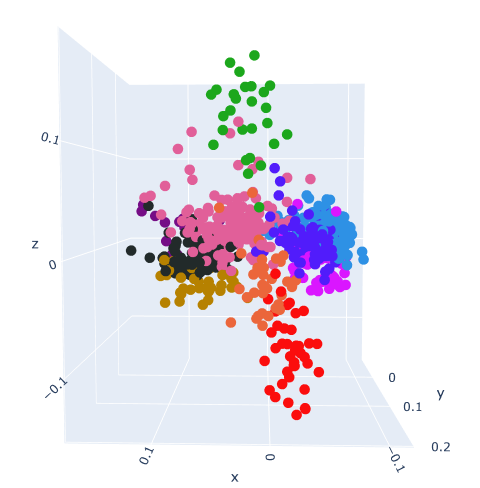
\includegraphics[width=0.8\textwidth]{figures/embeddings/embedding-lab.png}
      \caption{Visualize an example of a neural manifold generated from neural spiking data.}
      \label{fig:neural-manifold-eg}
            \end{figure} 
            
\section{How to generate the neural manifold?}
The task of generating the neural manifold is equivalent to learning\footnote{``Learning" here refers to unsupervised learning, which is a class of approaches in machine learning that discover meaningful features without training data.} the low-dimensional manifold underlying the original high-dimensional neural spiking data, which amounts to a dimensionality reduction task. In our project, we use both the linear dimensionality reduction method tensor canonical polyadic (CP) decomposition and the non-linear dimensionality reduction method diffusion map. The theoretical preliminaries for these two methods will be explained in full details in the next two chapters.

\section{What can we analyze from the neural manifold?}

We can directly compare the low-dimensional neural manifold for the biological neural networks with that for the artificial neural networks. The neural manifolds implies a functional network. The functional network is represented by the discrete data graph underlying the continuous manifold and thus reflects both the neural circuit connections and the neuron’s role in the circuit. We can thus make precise inferences about the similarities and differences between the particular biological and artificial neural networks in terms of their respective functional circuit, which is what we set out to compare. 


We can further extend this comparison to the \textit{topological} properties of the neural manifolds by extracting the topological features via persistent homology and quantifying the topological similarities using appropriate distance metric between the topological features. In our study, we have chosen the commonly used $p$-Wasserstein distance to quantify the pairwise similarities between the topological features of the neural manifolds given different stimuli. 

The following flowchart showed a schematic summary of the methodology of the project.

\bigskip

\begin{tikzpicture}[font={\sf \small}]
 \def\smbwd{2cm}
  \node (BNN) at (-3.6,0.5) [draw, terminal, minimum width=\smbwd,  fill=yellow!20, minimum height=0.5cm] {Biological Neural Networks}; 
  \node (ANN) at (3.5,0.5) [draw, terminal, minimum width=\smbwd,  fill=yellow!20, minimum height=0.5cm] {Artificial Neural Networks}; 
  %------------
  \node (experimental) at (-3.6,-1) [draw, terminal, minimum width=\smbwd,  fill=red!20, minimum height=0.5cm]{Neural population response (lab)};
  \node (artificial) at (3.5,-1)[draw, terminal,minimum width=\smbwd,  fill=red!20, minimum height=0.5cm]{Neural population response (simulations)};
  %------------
  \node (tensors) at (-1,-2) [draw, terminal, minimum width=\smbwd,  fill=red!20, minimum height=0.5cm] {Neural tensors}; 
  %------------
  
  \node (TCA) at (-3,-3.7) [draw, process, minimum width=\smbwd, fill=blue!20, minimum height=0.7cm] {Tensor CP decomposition};
  \node (diffusion) at (2,-3.5) [draw, process, minimum width=\smbwd, fill=blue!20, minimum height=0.7cm] {Diffusion map};
  %------------
  
  \node (manifolds) at (-1,-5) [draw, terminal, minimum width=\smbwd,  fill=green!20, minimum height=0.5cm] {Neural manifold};
  
  \node (TDA) at (-1,-6.5) [draw, process, minimum width=\smbwd, fill=blue!20, minimum height=0.7cm] {Topological Data Analysis};
   
 \node (topology) at (-1,-8) [draw, terminal, minimum width=\smbwd,  fill=green!20, minimum height=0.5cm] {Topological features};
 
  %------------
 
 \path [line](BNN) -- (experimental);
 \path [line](ANN) -- (artificial);
 \path [line](tensors) -- (TCA);
 \path [line](tensors) -- (diffusion);
 \path [line](experimental) -- (tensors) ;
 \path [line] (artificial) -- (tensors) ;
 \path [line](diffusion) -- (manifolds);
 \path [line](TCA) -- (manifolds);
  \path [line](manifolds) -- (TDA);
  \path [line](TDA) -- (topology);
 \end{tikzpicture}
 
 % 

% Consider a set of $N$ neurons responding to a specific sensory signal associated with an object. The neural population response to that stimulus is a vector in $\mathbb{R}^N$. 

% We model a set of $P$ manifolds corresponding to $P$ objects.
% Each manifold $M_\mu$ for $\mu 1, \dots, P$ consists of a compact
% subset of an affine subspace of $\mathbb{R}^N$ with affine dimension $D$ with $D < N$. A point on the manifold $x_\mu \in M_\mu$ can be parametrized as
% \begin{align}
%     \xx^\mu(\vec{S}) = \sum_{i = 1}^{D+1} S_i \uu^\mu_i
% \end{align}
% (Notations adapted from \cite{chung_classification_2018})